\section{Kiến trúc bộ phát}\label{IIA}

Quá trình thực hiện mã hóa và giả mã IDMA của $N$ STAs được diễn tả ở Hình \ref{fig:IDMASystem}, trong đó khối trãi tín hiệu và đan xen là hai quá trình quan trọng khi thực hiện IDMA \cite{IDMA_LiPing}. Dữ liệu $d_n$ của mỗi STA được trãi ra bởi chuỗi chip $c$ = [-1 1 $\dots$ -1 1], với \acrshort{SF} là hệ số trãi với giá trị bằng chiều dài của chuỗi chip. Điều kiện tiên quyết để IDMA hoạt động là mỗi STA thứ $n$ sẽ được trộn bởi một mã đan xen riêng biệt $\pi_n$, giả sử chuỗi $\pi_n$ là ngẫu nhiên độc lập với nhau.

\section{Kiến trúc bộ thu}\label{IIB}

Tín hiệu nhận được ở phía thu có thể được công thức hóa bởi \eqref{eq:1}, với tín hiệu phát và thu tương ứng với $[\mathbf{x}_1 \cdots \mathbf{x}_N]^\top$ và $[\mathbf{y}_1 \cdots \mathbf{y}_K]^\top$. $\mathbf{x}_n$ là vector tín hiệu của STA thứ $n$, $\mathbf{y}_k$ là vector tín hiệu nhận tại ăng-ten thứ $k$ của AP và nhiễu phía thu tại ăng-ten theo phân phối Gauss phức với $\mathbf{N} \sim \mathcal{N}_\mathbb{C}(\mathbf{0},\sigma^2\mathbf{I}_K)$

\begin{equation}
    \begin{bmatrix}
        \mathbf{y}_1 \\
        \vdots       \\
        \mathbf{y}_K \\ 
    \end{bmatrix}
    =
    \begin{bmatrix}
        \mathbf{h}_{1,1}  & \cdots & \mathbf{h}_{1,N} \\
        \vdots            & \ddots & \vdots           \\
        \mathbf{h}_{K,1}  & \cdots & \mathbf{h}_{K,N} 
    \end{bmatrix}
    \times
    \begin{bmatrix}
        \mathbf{x}_1 \\
        \vdots       \\
        \mathbf{x}_N \\ 
    \end{bmatrix}
    +
    \mathbf{N}.
    \label{eq:1}
\end{equation}

Thành phần chính yếu trong bộ giải mã IDMA chính là \acrfull{ESE} được dùng để tính toán tỉ số \acrfull{LLR} cho vector tín hiệu $\mathbf{x}_n $ = $[x_n(1),\dots,x_n(j),\dots,x_n(J)]$ của STA thứ $n$ STA và bộ giải mã dựa trên xác xuất hậu nghiệm \acrfull{APP}.

\subsection{Elementary Signal Estimator} \label{sub2.1}

Vector tín hiệu tại ăng-ten thứ $k$ có thể được viết lại như \eqref{eq:2}

\begin{figure}
    \centering
    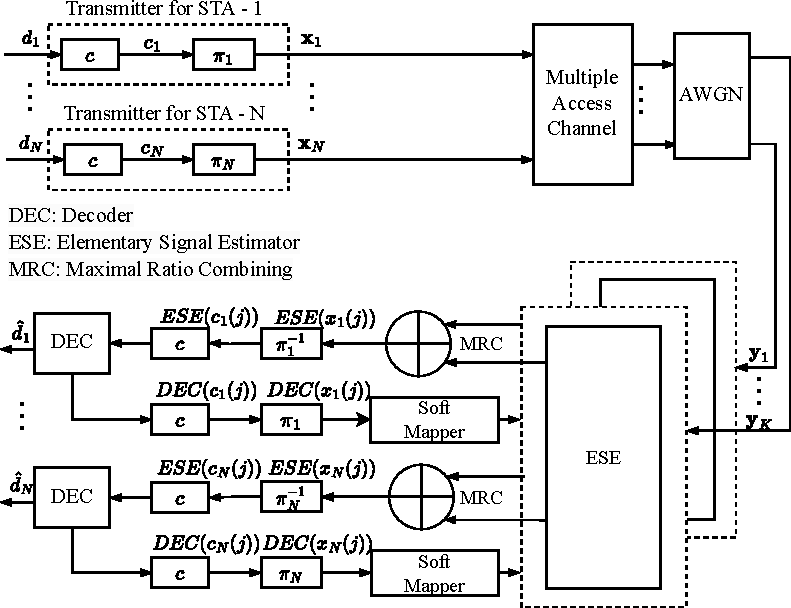
\includegraphics[width = 0.75\linewidth]{figure/Chap2/IDMA_Tx_Rx_structure-2_k2opt.pdf}
    \caption{Hệ thống IDMA với đa ăng-ten nhận.}
    \vspace{-1em}
    \label{fig:IDMASystem}
\end{figure}

\begin{equation}
    \mathbf{y}_k = \mathbf{h}_{k,n} \times \mathbf{x}_n 
    + \overbrace{\sum_{n' \neq n}\mathbf{h}_{k,n'} \times \mathbf{x}_{n'} 
    + \mathbf{N}}^{\zeta_{k,n}},
    \label{eq:2}
\end{equation}%\vspace{-0.5em}
trong đó $\zeta_{k,n}$ là thành phần nhiễu cộng can nhiễu tại ăng-ten $k$. Từ định lý giới hạn trung tâm, ta có thể xấp xỉ $\zeta_{k,n}$ như một biến ngẫu nhiên có phần bố Gaus, và tín hiệu $\mathbf{y}_k$ có thể ghi như hàm PDF như \eqref{eq:3}
\begin{equation}
    % \begin{split}
         p(y_k(j)\mid x_n(j)=\pm 1) = 
         \frac{1}{\sqrt{2\pi}\text{Var}(\zeta_{k,n}(j))} 
        e^{\mathord{-}\dfrac{(y_k(j)\mathord{-}(\pm h_{k,n}(j)\mathord{+}\mathbb{E}(\zeta_{k,n}(j))))^2}{2\text{Var}(\zeta_{k,n}(j))}},
    % \end{split}
    \label{eq:3}
\end{equation}
trong đó $\mathbb{E}\{\cdot\}$ và Var$\{\cdot\}$ tương ứng là giá trị ky vọng và phương sai của phân bố. Định lý giới hạn trung tâm đúng khi áp dụng cho một lượng lớn phân bố ngẫu nhiên độc lập với nhau, và nó thích hợp để dùng trong IDMA. Thuật toán \ref{alg:ESE} với đầu vào là $\mathbf{y}_k$ và $\mathbf{h}_{k,n}$ được dùng để tính toán tỉ số LLR $x_{k,n}(j)$, với $\{\cdot\}^*$ và $\{\cdot\}^\top$ lần lượt là phép chuyển vị phức và phép chuyển vị.

Thuật toán \ref{alg:ESE} tính toán giá trị ESE cho STA thứ $n$ tại ăng-ten $k$ và các giá trị này sẽ được tính lại sau mỗi lần lặp, phần cập nhập sẽ được nói rõ ở phần \ref{update}.
Giá trị bit $b_{I,\nu}$ được quyết định cứng là $\beta$ (tương tự cho $b_{Q,\nu}$) được cho bởi
\begin{equation}
    p(b_{I,\nu} = \beta \mid y_{k,n}(j)) > p(b_{I,\nu} = (1-\beta) \mid y_{k,n}(j)). \label{eq:4}
\end{equation}

\begin{algorithm}
    % \vspace{-0.5em}
    \caption{ESE Detection Algorithm.}\label{alg:ESE}
    % \footnotesize
    \begin{algorithmic}[1]
        \Procedure{ESE}{$\mathbf{y}_k,\mathbf{h}_{k,n}$} 
    
            % \While{$j \leq J$}               
                \State $\mathbb{E}(x_{k,n}(j)) = 0$     \Comment{Khởi tạo ban đầu}
    
                \State $\mathbb{E}(y_{k,n}(j)) = 0$
    
                \State $\textbf{Cov}(x_{k,n}(j)) = \textbf{I}_2$
                \State $\textbf{Cov}(y_{k,n}(j)) = \sigma^2\textbf{I}_2$
    
                \State $\textbf{R}_{k,n}(j)=
                \begin{bmatrix}
                    \Re(h_{k,n}(j))   & -\Im(h_{k,n}(j))  \\ 
                    \Im(h_{k,n}(j))   & \Re(h_{k,n}(j))
                \end{bmatrix}$
    
                \State $\textbf{Cov}(\zeta_{k,n}(j))=\textbf{Cov}(y_{k,n}(j))~-~\textbf{R}_{k,n}(j)\textbf{Cov}(x_{k,n}(j)) \textbf{R}_{k,n}(j)^\top$
    
                \State $\text{Var}(\tilde{\zeta}_{k,n}(j)) = \textbf{R}_{k,n}(j)^\top \textbf{Cov}(\zeta_{k,n}(j)) \textbf{R}_{k,n}(j)$
    
                \State $\mathbb{E}(\tilde{\zeta}_{k,n}(j)) = h_{k,n}^{*}(j)(\mathbb{E}(y_{k,n}(j)) - h_{k,n}(j) \mathbb{E}(x_{k,n}(j)))$
    
                \State $ESE(x_{k,n}(j))~=~\dfrac{2\lvert h_{k,n}\rvert^2\overbrace{(h_{k,n}^{*}(j) y_{k,n}(j) - \mathbb{E}(\tilde{\zeta}_{k,n}(j)))}^{LLR}}{\text{Var}(\tilde{\zeta}_{k,n}(j))}$                                  \Comment{Tính toán ESE}
    
            % \EndWhile  
    
        \EndProcedure
    \end{algorithmic}
\end{algorithm}

Tỉ số LLR được tính bởi
\begin{equation}
    % \begin{split}
         LLR(b_{I,\nu})  \triangleq \log \left(\dfrac{p(b_{I,\nu} \mathord{=} 1 \mid y_{k,n}(j))}{p(b_{I,\nu} \mathord{=} 0 \mid y_{k,n}(j))}\right)
         \mathord{=} \log \left(\dfrac{\sum_{\alpha\in S_{I,\nu}^{(1)}}p(x_{k,n}(j)\mathord{=} \alpha\mid y_{k,n}(j))}{\sum_{\alpha\in S_{I,\nu}^{(0)}}p(x_{k,n}(j)\mathord{=} \alpha\mid y_{k,n}(j))}\right),
    % \end{split}
    \label{eq:5}
\end{equation}
sử dụng lý thuyết Baye và giả sử các symbol có phân phối như nhau, \eqref{eq:5} được viết lại
\begin{equation}
    LLR(b_{I,\nu})\mathord{=}\log \left(\dfrac{\sum_{\alpha\in S_{I,\nu}^{(1)}}p(y_{k,n}(j) \mid x_{k,n}(j)\mathord{=} \alpha)}
    {\sum_{\alpha\in S_{I,\nu}^{(0)}}p(y_{k,n}(j) \mid x_{k,n}(j)\mathord{=} \alpha)}\right).
    \label{eq:6}
\end{equation}

một bài toán tối ưu để tính tỉ số LLR một cách đơn giản hơn khi dùng khai triển Taylor cho biểu thức $\log (1+z)$ khi $z \ll 1$, dễ dàng thấy được: $\log \Sigma_jz_j \approx \text{max}_j \log z_j$, khi đó \eqref{eq:6} được viết gần đúng bởi \eqref{eq:7}
\begin{equation}
    LLR(b_{I,\nu}) \mathord{\approx}\log \left(\dfrac{\max_{\alpha\in S_{I,\nu}^{(1)}} p(y_{k,n}(j) \mathord{\mid} x_{k,n}(j)\mathord{=} \alpha)}
    {\max_{\alpha\in S_{I,\nu}^{(0)}} p(y_{k,n}(j) \mathord{\mid} x_{k,n}(j)\mathord{=} \alpha)}\right),
    \label{eq:7}
\end{equation}
với $\alpha$ là một điểm trên chòm sao. Hình \ref{fig:16-QAM} cho thấy vùng quyết định $S_{I,\nu}^{(s)}$ cho thành phần thực $b_{I,\nu}$ và $S_{Q,\nu}^{(s)}$ cho thành phần ảo $b_{Q,\nu}$ với $s=[0,1]$ trong trường hợp 16-QAM. Dễ dàng nhận thấy chúng được phân định bởi ranh giới ngang hoặc dọc. Do đó, hai ký hiệu trong hai tập con gần tín hiệu cân bằng nhận được nhất luôn nằm trên cùng một hàng nếu ranh giới phân vùng là dọc (bit $b_{I,1}$ và $b_{I,2}$ trong Hình \ref{fig:16-QAM}) hoặc trong cùng một cột nếu ranh giới nằm ngang (bit $b_{Q,1}$ và $b_{Q,2}$ trong Hình \ref{fig:16-QAM}). Kết quả là, khi sử dụng \eqref{eq:3} trong \eqref{eq:7}, các giá trị bit mềm cuối cùng có thể được biểu thị bằng khoảng cách Euclide tối thiểu như sau
\begin{equation}
    \begin{split}
        LLR(b_{I,\nu}) =&\dfrac{\absolutevalue{h_{k,n}(j)}^2}{4} \Bigg\{ \min_{\alpha_I \in S_{I,\nu}^{'(0)}}(\Re(y_{k,n}(j)) - \alpha_I)^2 - \min_{\alpha_I \in S_{I,\nu}^{'(1)}}(\Re(y_{k,n}(j)) - \alpha_I)^2 \Bigg\}\\
        \triangleq & \absolutevalue{h_{k,n}(j)}^2 \times D_{I,\nu}, 
    \end{split}
    \label{eq:8}
\end{equation}
trong đó $S_{I,\nu}^{'(s)} \triangleq \Re(S_{I,\nu}^{(s)})$.

\begin{figure}
    \centering
        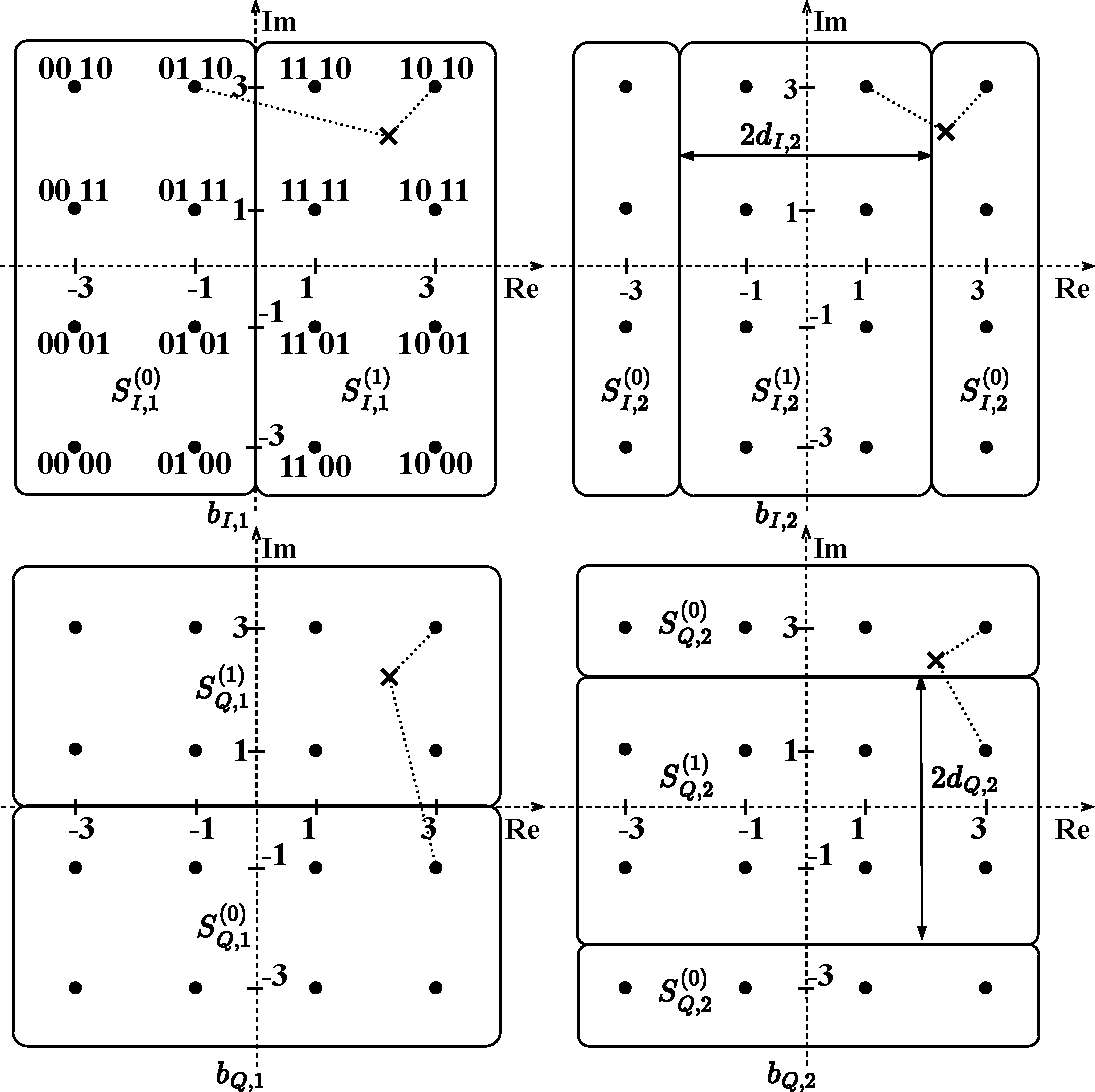
\includegraphics[width=0.75\linewidth]{figure/Chap2/16-QAM.pdf}
    \caption{Giải điểu biến 16-QAM đơn giản.}
    \label{fig:16-QAM}
    \vspace{-1em}
\end{figure}

Việc tính toán chính xác $D_{I,\nu}$, $D_{Q,\nu}$ trong \eqref{eq:8} yêu cầu nhiều phép tính của hàm logarit và việc thực hiện phức tạp hơn. Bài viết này triển khai \cite{SimpleDemap} để tính giá trị LLR gần đúng. Các giá trị $D_{I,\nu}$ và $D_{Q,\nu}$ cho 16-QAM được tính bởi
\begin{equation}
    D_{I,1}=\left\{
        \begin{matrix}
            2\Re(y_{I,k,n}(j))+2 & \Re(y_{k,n}(j)) < -2, \\ 
             \Re(y_{I,k,n}(j))   & -2\leq \Re(y_{k,n}(j)) \leq 2, \\ 
            2\Re(y_{I,k,n}(j))-2 & \Re(y_{k,n}(j)) > 2, 
        \end{matrix}
    \right. \label{eq:9}
\end{equation}
\begin{equation}
    \begin{matrix}
        D_{I,2}=-\absolutevalue{\Re(y_{I,k,n})} & \text{for all } \Re(y_{I,k,n}).
    \end{matrix}
    \label{eq:10}
\end{equation}

Thay thế phần $LLR$ ở dòng 10 trong thuật toán \ref{alg:ESE} bằng \eqref{eq:8}, công thức $ESE$ có thể được biểu diễn dưới dạng 
\begin{equation}
    ESE(\Re(x_{k,n}(j)))~=~\dfrac{2\lvert h_{k,n}\rvert^4D_{I,\nu}}
    {\text{Var}(\tilde{\zeta}_{k,n}(j))},
\end{equation}  
và $ESE(\Im(x_{k,and}(j)))$ được tính theo cách tương tự.


\subsection{Khối DEC}

Sau khi tính toán giá trị LLR, báo cáo này sử dụng kỹ thuật \acrshort{MRC} để đat tỷ số tín hiệu trên nhiễu \acrshort{SNR} cao nhất có thể đạt được tại AP. Sau đó, quá trình loại bỏ xen kẽ sẽ được thực hiện với cùng mã bộ xen $\pi_n$, được sử dụng cho STA thứ $n$ tại máy phát. Tiếp theo, giá trị chip LLR được so sánh với ngưỡng. Nếu các giá trị này lớn hơn ngưỡng, chúng sẽ bị cắt bớt thành giá trị ngưỡng.

\subsection{Cập nhật giá trị trung bình và phương sai} \label{update}
Sau khi tính toán DEC, IDMA cần cập nhật giá trị trung bình và phương sai cho lần lặp tiếp theo. Phần cập nhật bao gồm bộ trãi mã, bộ xen kẽ và bộ ánh xạ mềm. Đầu ra của quá trình khử trải phổ là các LLR bên ngoài cho $y_{k,n}(j)$ Sau đó, các LLR này được sử dụng để tạo số liệu thống kê trong \eqref{eq:12}, \eqref{eq:13}
\begin{equation}
    \mathbb{E}(x_{k,n}(j)) = \sum_{\nu = 0}^{2^{N_{bpsc}}-1} (p \mathord{+}iq)_\nu \mathord{\times} \left(\dfrac{e^{DEC(\hat{a}_n(j))}}{1 \mathord{+} e^{DEC(\hat{a}_n(j))}}\right)_\nu,
    \label{eq:12}
\end{equation}
\begin{equation}
    % \begin{split}
        \textbf{Cov}(x_{k,n}(j))
        =\textbf{I}_2 \mathord{\times}         
        \begin{bmatrix}
            \Re(\text{Var}(x_{k,n}(j))) \mathord{-} \Re(\mathbb{E}(x_{k,n}(j)))^2 \\
            \Im(\text{Var}(x_{k,n}(j))) \mathord{-} \Im(\mathbb{E}(x_{k,n}(j)))^2
        \end{bmatrix},
    % \end{split}
    \label{eq:13}
\end{equation}
trong đó $N_{bpsc}$ là số bit trên mỗi ký hiệu, $p$ và $q$ là các giá trị được lấy bởi trục $\Re$ và $\Im$ (ví dụ: các giá trị là $\{$-3, -1, +1, +3$\}$ cho 16-QAM).
